%part 2

	\chapter{Прохождение критической энергии в регулярной магнитооптической структуре синхротрона}\label{ch:transition}

\par Данная глава посвящена рассмотрению влияния критической энергии на продольную динамику, а также процедуры скачка критической энергии в регулярной структуре синхротрона.

\par Исходя из изложенных уравнений продольного движения в Главе \ref{ch:dual}, приближение энергии пучка к критическому значению ведет к изохронному движению, при котором частота синхротнонных колебаний стремится к нулю и означает отсутствие продольное перемешивания частиц в сепаратрисе. При этом теряется фазовая стабильность, нарушается адиабатичность движения, а также проявляется влияние высших порядков зависисмоти от разброса по импульсу – нелинейность.

\par Увеличение скорости прохождения критической энергии уменьшает влияние факторов, возмущающих фазовое движение. Широко используется метод скачка критической энергии, который применяется на многих установках CERN \cite{risselada:jump}, BNL \cite{ainsworth:pip}, в том числе был реализован в России на синхротроне У-70 \cite{u-70}. Сдвиг критической энергии обеспечивается искажением дисперсионной функции за счёт использования тонких квадрупольных линз \cite{u-70_jump}. Такой метод для каждой отдельной установки рассматривается отдельно и устанавливает ограничения в зависимости от потребностей конечного эксперимента.

\par Прохождение критической энергии является актуальной задачей для протонного пучка в строящемся комплексе NICA (ОИЯИ г. Дубна). С целью изучения данной проблемы, исследована динамика продольного движения в окрестности критической энергии У-70 (НИЦ “Курчатовский институт” - ИФВЭ г. Протвино).  Промоделирована процедура скачка критической энергией в синхротроне У-70 при помощи численного моделирования. Полученные данные также апробированы на ускорительном сеансе. \cite{?}

\par Важным фактором, описывающим взаимодействие пучка и элементов ускорителя является влияние различного рода импедансов, а также типо высокочастотных резонаторов (ВЧ) на продольную динамику во время процедуры преодоления критической энергии. Отличительной особенностью является использование ВЧ барьерного типа, в результате чего достигается специфическое распределение пучка в фазовом пространстве, отличное от классического, формируемого гармоническим ВЧ.

\par Результаты данного исследования помогут осветить потенциальные последствия прохождения критической энергии и определить существенные параметры, влияющие на динамику фазового движения.

	\section{Построение регулярной структуры на основе ячеек ФОДО, ФДО, ОДФДО}\label{sec:transition_jump/FODO_FDO}

\par На основе ФОДО, ФДО и ОДФДО ячеек могут быть сконструированы регулярные поворотные арки как показано на рис. \ref{fig:fodo_fdo_odfdo_regular}.

\begin{figure} [h!]

   \includegraphics*[width=.32\columnwidth]{2_twiss_fodo_cell.pdf}
   \includegraphics*[width=.32\columnwidth]{2_twiss_fdo_cell.pdf}
   \includegraphics*[width=.32\columnwidth]{2_twiss_odfdo_cell.pdf}

   \includegraphics*[width=.32\columnwidth]{2_twiss_fodo_regular.pdf}
   \includegraphics*[width=.32\columnwidth]{2_twiss_fdo_regular.pdf}
   \includegraphics*[width=.32\columnwidth]{2_twiss_odfdo_regular.pdf}

   \caption{Твисс-параметры $\beta_{x,y}$, $D_{x}$. Сверху -- для ячеек для сигнлетной ФОДО, дублетной ФДО, триплетной ОДФДО ячеек; посредине -- регулярная структура; снизу -- резонансная.}
   \label{fig:fodo_fdo_odfdo_regular}
\end{figure}

\par Для ФОДО ячейки характерно максимальное простраственное разделение минимумов и максимумов бета-функций. Однако, макмиальное значение бета-функции и дисперсионной функции наибольшее для ФОДО структуры. Также стоит отметить, что растет градиент в квадрупольных линзах для постижения одинакового набега фазы, в таком порядке ФОДО, ФДО, ОДФДО. 

	\subsection{Подавление дисперсии в регулярных арках с missing magnet и/или квадруполями с варьируемыми градиентами}\label{sec:transition_jump/suppression}

\par Подавление дисперсии используется для ряда задач в ускорительной технике.
	
\par Для коллайдерных экспериментов, необходимо в точке встречи (Interaction Point - IP) иметь нулевое значение дисперсионной функции, так как два пучка должны столкнуться в определенной заданной точке для достижения большой светимости.

\par Также это может применяться при инжекции из бустера (buster) в основное кольцо (main ring), поскольку. Иначе нужно каким-то сложным образом нарочно возбуждать орбиту и делать её ненулевой, чтобы произошёл точное совпадение твисс-функций при инжекции. 

\par В случае спиновой динамики, на прямом участке необходимо использование фильтров Вина. Такое устройство не возмущает орбиту так как изначально планируется сделать нулевую силу Лоренца (или одинаковую кривизну полей E и B полей). При этом искажается дисперсионная функцыия, что должно быть компенсировано магнитами. При движение частиц по смещенной траектории, возникает  действие полей, которое будет нескомпенсированно.

\par При всём этом для NICA инжекция происходит в место с ненулевой дисперсией , это обусловлено особенностью расположения оборудования.
	
	\section{Прохождение критической энергии}\label{sec:transition_jump/U-70}
	
	\subsection{Численное моделирование динамики продольного движения} \label{sec:transition_jump/modeling}
	
\par Основные уравнения, которые будут проанализированы – уравнения продольного фазового движения.
Наиболее классически уравнения \ref{eq:long_motion_eq_n} могут быть записаны в зависимости от времени:
	
\begin{equation}
\begin{cases}
\begin{aligned}
& \frac{d \tau}{d t}=\eta(\delta) \cdot \frac{h \cdot \Delta E}{\beta^2 \cdot E_0} \\
& \frac{d(\Delta E)}{d t}=\frac{V(\tau)}{T_0}
\end{aligned}
\end{cases}
\label{eq:long_motion_eq_t}
\end{equation}	

\noindent Для моделирования приведенной системы уравнений используются различные программы. Наиболее современной является BLonD \cite{blond}, CERN. Для пересчёта временной задержки могут быть использованы 2 различные схемы, как 'простая', учитывающая только первый порядок разложения $\eta$:

\begin{equation}
\Delta t^{n+1}=\Delta t^n+\frac{\eta_0^{n+1} T_0^{n+1}}{\left(\beta_s^{n+1}\right)^2 E_s^{n+1}} \Delta E^{n+1},
\label{eq:blond_dt_simple}
\end{equation}

\noindent так и 'точная', учитывающая зависимость от высших порядков разложения: 

\begin{equation} \label{eq:blond_dt_exact}
\begin{aligned}
 \Delta & t^{n+1}=\Delta t^n+T_0^{n+1}\times\\
& \times \left[\left(1+\alpha_0^{n+1} \delta^{n+1}+\alpha_1^{n+1}\left(\delta^{n+1}\right)^2+
\alpha_2^{n+1}\left(\delta^{n+1}\right)^3\right)\left(\frac{1+\frac{\Delta E^{n+1}}{E_s^{n+1}}}{1+\delta^{n+1}}\right)-1\right].
\end{aligned}
\end{equation}

\noindent Для пересчёта приращения энергии используется уравнение:

\begin{equation} \label{eq:blond_dE}
\Delta E^{n+1}=\Delta E^n+\sum_{k=0}^{n_{\mathrm{rf}-1}-1} V_k^n \sin \varphi_{\mathrm{rf}, k}\left(\Delta t^n\right)-\left(E_s^{n+1}-E_s^n\right)
\end{equation}

\noindent как видно из ур. \ref{eq:blond_dE} ускорение может быть обеспечено влиянием только гармонического ВЧ. Такой подход создаёт сложности при необходимости моделирования в BLonD барьерного ВЧ, тогда необходимо представить в виде набора ВЧ станции с различными частотами, соответствующим Фурье-разложению потенциального барьера сигнала.
	
	\subsection{Стабильность продольного фазового движения вблизи критической энергии}\label{sec:transition_jump/adiabaticity}
	
\par Уравнения \ref{eq:long_motion_eq_t} определяют продольные колебания с определенной частотой. Вдали от критической энергии частота синхротронных колебаний слабо меняется со временем, движение адиабатично. Вблизи критической энергии нарушается условие адиабатичности синхротронного движения. Характерное время адиабатичности можно оценить, сравнивая синхротронную частоту с темпом изменения удерживающей сепаратрисы, что показано на рис. \ref{fig:adiabatic_time_nonlin_time}a \cite{ng}:

\begin{equation}
\tau_{ad}=\left(\frac{\pi\beta^2mc^2\gamma_{tr}^4}{\dot{\gamma}\omega_0^2heV\left|\cos{\phi_s}\right|}\right)^{1/3}
\label{eq:adiabaticity}
\end{equation}

\noindent где $\gamma_{tr}$ – Лоренц-фактор, соответствующий критической энергии, $\dot{\gamma}$ – темп изменения энергии. При адиабатичном движении как сепаратриса, так и частота колебаний медленно меняется со временем.

\par Нелинейность продольного движения проявляется, когда $\eta_1\delta$ сравнимо с $\eta_0$, характерное время (рис. \ref{fig:adiabatic_time_nonlin_time}б):

\begin{equation}
\tau_{nl}=\frac{\eta_1\hat{\delta}}{\sfrac{2\dot{\gamma}}{{\gamma_{tr}}^3}}=\gamma_{tr}\frac{\sfrac{3}{2}\beta^2+\gamma_{tr}^2\alpha_1}{2\dot{\gamma}}\
\label{eq:nonliniarity}
\end{equation}

\noindent где $\hat{\delta}\approx{10}^{-2}-{10}^{-3}$ – абсолютное значение максимального отклонения импульса вблизи критической энергии, $\alpha_1$ – второй порядок коэффициента уплотнения орбиты. Для регулярной ФОДО структуры У-70 с скомпенсированной натуральной хроматичностью, получено $\alpha_1\simeq0.01$ [6].

\begin{figure}
   \includegraphics*[width=0.49\columnwidth]{3_adiabatic_time.png}
   \includegraphics*[width=0.49\columnwidth]{3_nonlin_time.png}
   \caption{а) Классическая синхротронная частота и тем изменения огибающей сепаратрисы в окресности критической энергии от номера оборота; б) изменение первого и второго порядка коэффициента проскальзывания $\eta_0$, $\eta_1\delta$ в окресности критической энергии от номера оборота.}
   \label{fig:adiabatic_time_nonlin_time}
\end{figure}

\par Кроме того, из ур. \ref{eq:long_motion_eq_t} следует условие стабильности синхротронных колебаний

\begin{equation}
\eta_0\cos\phi_s<0
\label{eq:long_stability}
\end{equation}

\noindent Видно, что для продольного согласования при прохождении критической энергии также должна быть сдвинута фаза $\phi_s$ ускоряющего поля ВЧ на $\pi-2\phi_s$.

\begin{figure}
   \includegraphics*[width=0.32\columnwidth]{3_eta_beam_lenght.png}
   \includegraphics*[width=0.32\columnwidth]{3_eta_energy_spread.png}
   \includegraphics*[width=0.32\columnwidth]{3_eta_emit.png}
   \caption{Зависимость a) длины cгустка, б) разброса энергии внутри сгустка, в) продольного эмиттанса от номера оборота в окрестности критической энергии при изменении энергии от $7$ до $13$ ГэВ для трёх моделей без скачка и учёта импеданса. 
Синяя – учёт только первого порядка $\eta=\eta_0$, ‘simple’ solver, оранжевая – $\eta=\eta_0$, ‘exact’ solver, зеленая – $\eta=\eta_0+\eta_1\delta$, ‘exact’ solver.}
   \label{fig:3_eta}
\end{figure}

\par Оценки для У-70, приведенные в табл. 1, отражают тот факт, что время адиабатичности (2) может быть сравнимо со временем нелинейности (3) $\tau_{ad}\sim\tau_{nl}$. При приближении энергии к критической, продольная длина пучка уменьшается, а разброс по импульсам увеличивается. На рис. 2 приведены результаты моделирования прохождения критической энергии при ускорении от $7.0$ до $13.0$ ГэВ для $\eta=\eta_0$ и $\eta=\eta_0+\eta_1\delta$ в различных моделях BLonD. Влияние второго порядка коэффициента проскальзывания увеличивает продольный эмиттанс.

\subsection{Влияние индуктивного импеданса}

\par На продольную динамику также оказывает влияние элементы ускорителя. Для описания электромагнитного взаимодействия пучка с элементами структуры ускорителя вводится понятие импеданса. И обычно может являться достаточно сложной функцией, содержащей как мнимую, так и действительную часть. Вид импеданса может быть определен как аналитически, взяв во внимание все наиболее значимые элементы, так и экспериментально, на уже действующей установке. Поскольку оба эти подхода являются достаточно комплексными и сложными, в качестве первого приближения могут быть использованы более простые модели импедансов.
\par Особенно важным для изучения продольной динамики при прохождении критической энергии является продольный импеданс $Z_\parallel\left(\omega\right)$. В данной работе ограничимся исследованием динамики с учётом его мнимой индуктивной компонентой $\sfrac{Z_n}{n}=\pm i \cdot const$. Положительная индуктивность может соответствовать продольному импедансу связи пикап-электродов, кикер-магнитов и сильфонов [3]. Отрицательная индуктивность соответствует импедансу гладкой камеры при наличии пространственного заряда \cite{laclare} и описывается аналитически:

\begin{equation}
\frac{Z_{SC}}{n}=-\frac{Z_0}{2\beta\gamma^2}\left[1+2\ln{\left(\frac{b}{a}\right)}\right].
\label{sc}
\end{equation}

\noindent Для наглядности, приведём напряжение, индуцированное про\-стран\-стве\-нным зарядом, $V_{\mathrm{s.c.\ }}(\phi)$. Уравнение определяется производной от функции распределения $f(\phi)$ в пространстве \cite{sc}:

\begin{equation} \label{V_sc}
V_{\text{S.C.}}\left(\phi\right)=\frac{Z^2h^2g_0Z_0ce}{2R_0\gamma^2}\cdot\frac{\partial\left(N_0f\left(\phi\right)\right)}{\partial\phi}.
\end{equation}

\par На сеансе для У-70 наблюдалась интенсивность в импульсе порядка $N_{tot}=4\cdot{10}^{12}$ ppp (particles per period), соответственно, в сгустке – порядка $N_{beam}=4\cdot{10}^{11}$ ppb (particles per beam). Моделирование продольной динамики при изменении энергии от 7 до 9 ГэВ показывает, что при малой интенсивности $N_{beam}=4\cdot{10}^{11}$ ppb как для отрицательного, так и для положительного значений рассматриваемого импеданса пучок сохраняет стабильность. Для больших интенсивностей $N_{beam}=1\cdot{10}^{12}$ ppb наблюдается существенное изменение симметрии фазового объёма и увеличение продольного эмиттанса (рис. 3, табл. \ref{tbl:u-70_crossing}). В соответствии с экспериментальными данными начальное значение длины сгустка $\tau_L=4t_\sigma\simeq20$ нс для $E_0=7$ ГэВ. Для гауссова распределения $\delta E_{0} = 4E \sigma = 52.7$ МэВ, $\varepsilon_{0 95\%}=1.23$ эВ$\cdot$с.
	
\begin{figure} [h!]
   \includegraphics*[width=0.32\columnwidth]{3_wo_jump_beam_lenght.png}
   \includegraphics*[width=0.32\columnwidth]{3_wo_jump_energy_spread.png}
   \includegraphics*[width=0.32\columnwidth]{3_wo_jump_emit.png}
   \caption{Зависимость a) длины cгустка, б) разброса энергии внутри сгустка, в) продольного эмиттанса от номера оборота в окресности критической энергии при изменении энергии от $7$ до $9$ ГэВ без скачка, с учётом различного вида импеданса и интенсивностей.}
   \label{fig:3_wo_jump}
\end{figure}

\begin{table}
\begin{center}
\begin{tabular}{| m{4cm} | M{2.5cm} | M{2.5cm} | m{6.6cm} |}
\hline 
Параметры моделирования & $95 \%$ фазовый объем & Сохранение пучка & Особенности \\
\hline
$\alpha_1=0, \text { simple, }$ Без импеданса & 1.23 & $100\%$ & Простая модель, рост эмиттанса отсутствует \\
\hline 
$\alpha_1=0, \text { exact, }$ Без импеданса & 1.4 & $99.65\%$ & Точная модель, нелинейность отсутствует, влияние неадиабатичности, рост эмиттанса \\
\hline 
$\alpha_1=0.01, \text { exact, }$ Без импеданса & 1.8 & $99.65\%$ & Влияние нелинейности, рост эмиттанса в $\sim 1.5$ раза \\
\hline 
$
 \alpha_1=0.01, \text { exact, }$
$ Z_n / n=-i \cdot 10, \quad$
$4 \cdot 10^{11} \mathrm{ppb} $
 & 1.8 & $99.65\%$ & Уменьшение длины сгустка после $\gamma_{\mathrm{tr}}$, фокусирование после $\gamma_{\mathrm{tr}}$, рост эмиттанса \\
\hline 
$
\alpha_1=0.01, \text { exact, }$ 
$ Z_n / n=+i \cdot 10, \quad$
$4 \cdot 10^{11} \mathrm{ppb} $
 & 1.9 & $99.60\%$ & Уменьшение длины сгустка до $\gamma_{\mathrm{tr}}$, раскачивание после $\gamma_{\mathrm{tr}}$, рост эмиттанса \\
\hline 
$
\alpha_1=0.01, \text { exact, } $ 
$Z_n / n=-i \cdot 10, \quad$
$1 \cdot 10^{12} \mathrm{ppb}$
 & 2.3 & $99.60\%$ & Существенное сжатие длины сгустка до $\gamma_{\mathrm{tr}}$, рост эмиттанса \\
\hline 
$
 \alpha_1=0.01, \text { exact, } $ 
$ Z_n / n=+i \cdot 10, \quad$
$ 1 \cdot 10^{12} \mathrm{ppb}$
 & 4.1 & $98.60\%$ & Увеличенная амплитуда квадрупольных колебаний, существенный рост эмиттанса \\
\hline
\end{tabular}
\end{center}
\caption{Результаты численного моделирования прохождения критической энергии, в том числе с учётом влияния различных импедансов для различных интенсивностей.}
\label{tbl:u-70_crossing}
\end{table}

\subsection{Процедура скачка критической энергии}

\par Для сохранения стабильности продольного движения, продольный эмиттанс не должен расти при прохождении критической энергии. Для этого используется метод скачка критической энергии при приближении энергии пучка к критической энергии. Такой подход заключается в быстром изменении параметров ускорителя, при котором изменяется $\alpha$ пропорциональная $\gamma_{tr}$ . В общем случае, коэффициент расширения орбиты определяется как интеграл:

\begin{equation}
\alpha=\frac{1}{C} \int_0^{\mathrm{C}} \frac{D(s)}{\rho(s)} d s
\label{eq:alpha_general}
\end{equation}

\noindent где $s$ -- переменная длины ускорителя, $D\left(s\right)$ -- дисперсионная функция, $\rho\left(s\right)$ -- кривизна орбиты. Изменение коэффициента расширения орбиты в стационарной установке возможно при модулировании дисперсионной функции, так как $\rho\left(s\right)$ остается неизменной. 

\par Таким образом, возрастает скорость прохождения критической энергии, при этом сам темп ускорения не меняется. Параметры скачка могут быть определены при рассмотрении магнитооптической структуры и возможностью изменения тока в вспомогательных квадрупольных линзах, либо в квадруполях, расположенных в поворотных арках. Особенности обоих подходов будут рассмотрены далее на примере скачка критической энергии в синхротроне У-70, а также синхротрона NICA.

\section{Особенности процедуры скачка критической энергии в синхротроне У-70}

\par Модуляция дисперсионной функции в синхротроне У-70 осуществляется вспомогательными квадруполями во $2$-ом и $8$-ом блоках каждого суперпериода [9]. На рис. 4 изображены параметры Твисса для одного суперпериода, состоящего из 10 магнитных блоков с совмещённой функцией как для полностью регулярной структуры У-70, так и структуры с искаженной дисперсионной функцией [10].

\begin{figure} [h!]
   \includegraphics*[width=0.49\columnwidth]{3_twiss_U70_regular.png}
   \includegraphics*[width=0.49\columnwidth]{3_twiss_U70_modulated.png}
   \caption{Твисс-параметры $\beta_x,\beta_y, D_x$ для суперпериода У-70 a) регуляная структура; б) структура с модулированной дисперсией.}
   \label{fig:3_twiss_U70}
\end{figure}

\par Вспомогательные квадруполи расположены через полпериода $\Delta\nu_{x,y}=0.5\times0.5$ и имеют противоположные полярности. При такой модуляции дисперсии не происходит сдвига рабочей точки, поскольку действие одного квадруполя, подавляется другим в силу указанного набега фазы. В табл. 3 приведены значения рабочей точки в ходе процедуры поднятия критической энергии и скачка. Таким образом, поднятие критической энергии на переднем фронте происходит на $\Delta \gamma_{tr}=0.9$ за $36$ мс, а сам скачок — за $1$ мс на заднем фронте. Принципиальная схема процедуры, а также соответствующее изменение первого порядка коэффициента скольжения приведены на рис. 5. Процедура скачка на сеансе У-70 приведена на рис. 6а, продольная линейная плотность сгустка относительно фазы ВЧ в момент скачка отражена на рис. 6б

\begin{table}
\begin{center}
\begin{tabular}{| m{10cm} | M{2.5cm} |}
\hline Полная длина $L$, м  & 1483.699 \\
Коэффициент расширения орбиты $\alpha_0$ & 0.011120 \\
Коэффициент расширения орбиты $\alpha_1$ & 0.01 \\
Критическая энергия, ГэВ & 7.957 \\
Лоренц-фактор $\gamma_{\mathrm{tr}}$ & 7.48 \\
Максимальная интенсивность в сеансе, ppp & $4 \cdot 10^{12}$ \\
Ускоряющая фаза $\sin \left(\phi_{\mathrm{s}}\right.$ ) & $1 / 2$ \\
Время адиабатичности $\tau_{\mathrm{ad}}$, мс & 3.218 \\
Время нелинейности $\tau_{\mathrm{nl}}$, мс & 2.646 \\
Гармоническое число & 30 \\
Амплитуда ускоряющих станций, кВ & 10 \\
Количество ускоряющих станций & 40 \\
Темп ускорения $\dot{\gamma}, \mathrm{c}^{-1}$ & 42.7 \\
\hline
\end{tabular}
\end{center}
\caption{Основные параметры кольца и ВЧ для У-70}
\end{table}

\begin{figure}
   \includegraphics*[width=0.49\columnwidth]{3_gamma_transition_jump_U70.png}
   \includegraphics*[width=0.49\columnwidth]{3_eta0_jump_U70.png}
   \caption{a) Поднятие критической энергии при процедуре скачка; б) соответствующее изменение первого порядка коэффициента скольжения $\eta_0$.}
   \label{fig:3_gamma_transition_jump_U70}
\end{figure}

\par Данные моделирования продольного движения соответствуют изменению длины сгустка в ходе ускорительного цикла на сеансе У-70 (рис. 7). Результаты моделирования продольного движения (Рис. 8 и Таблица 4) показаны для разных моделей при ускорении от $6.9-12.9$ ГэВ [9] для скачка критической энергии. А также для скачка с учётом импедансов вида $\sfrac{Z_n}{n}=\pm i\cdot const$ и разных интенсивностей при ускорении $6.9-8.9$ ГэВ (Рис. 9). Начальные значения $\tau_L=4t_\sigma\simeq20$ нс при $E_0=6.9$ ГэВ, $\delta E_{0} = 4E \sigma =49.3$ МэВ,  $\varepsilon_{0 95\%}=1.16$ эВ$\cdot$с. 

\begin{figure}
   \includegraphics*[width=0.49\columnwidth]{3_jump_U70_oscilogram.png}
   \includegraphics*[width=0.49\columnwidth]{3_jump_U70_beam_profile.png}
   \caption{а) Скачок критической энергии на сеансе У-70. Зелная линия – сигнал с фазового датчика, фиолетовая – градиент в обмотках дополниительных квадруполей, голубая – сигнал с пикового детектора; б) Продольная линейная плотность сгустка относительно фазы ВЧ в момент скачка.}
   \label{fig:3_jump_U70_oscilogram}
\end{figure}

\begin{figure}
   \centering
   \includegraphics*[width=0.49\columnwidth]{3_jump_U70_beam_lenght.png}
   \caption{Изменение длины сгустка в ходе ускорительного цикла на сеансе У-70.}
   \label{fig:3_jump_U70_beam_lenght}
\end{figure}

\begin{figure}
   \includegraphics*[width=0.32\columnwidth]{3_jump_beam_lenght.png}
   \includegraphics*[width=0.32\columnwidth]{3_jump_energy_spread.png}
   \includegraphics*[width=0.32\columnwidth]{3_jump_emit.png}
   \caption{Зависимость a) длины cгустка, б) разброса энергии внутри сгустка, в) продольного эмиттанса от номера оборота в окрестности критической энергии при изменении энергии от $6.9$ до $12.9$ ГэВ для трёх моделей со скачком, без учёта импеданса. Синяя – учёт только первого порядка $\eta=\eta_0$, ‘simple’ solver, оранжевая – $\eta=\eta_0$, ‘exact’ solver, зеленая – $\eta=\eta_0+\eta_1\delta$, ‘exact’ solver.}
   \label{fig:3_jump}
\end{figure}

\begin{figure}
   \includegraphics*[width=0.32\columnwidth]{3_jump_imp_beam_lenght.png}
   \includegraphics*[width=0.32\columnwidth]{3_jump_imp_energy_spread.png}
   \includegraphics*[width=0.32\columnwidth]{3_jump_imp_emit.png}
   \caption{Зависимость a) длины cгустка, б) разброса энергии внутри сгустка, в) продольного эмиттанса от номера оборота в окресности критической энергии при изменении энергии от $6.9$ до $8.9$ ГэВ со скачком, с учётом различного вида импеданса и интенсивностей.}
   \label{fig:3_jump_imp}
\end{figure}

\begin{table}
\begin{center}
\begin{tabular}{| M{5cm} |c|c|}
\hline 
Время от момента инжекции, мс & Рабочая точка $v_{x, y}$ & Относительно скачка \\
\hline
290 & $9.921 \times 9.842$ & До процедуры \\
295 & $9.917 \times 9.808$ & Начало процедуры \\
310 & $9.849 \times 9.787$ & Середина процедуры \\
326 & $9.780 \times 9.771$ & Момент скачка \\
330 & $9.902 \times 9.809$ & После \\
\hline
\end{tabular}
\end{center}
\caption{Изменение рабочей точки в процессе процедуры скачка критической энергии на У-70.}
\end{table}

\par При сравнении двух рассмотренных способов прохождения критической энергии: без скачка критической энергии и со скачком, можно установить, что при скачке продольная длина сгустка сокращается меньше. Таким образом и рассмотренные импедансы меньше возмущают сгусток. Рост эмиттанса наблюдается только при рассмотрении интенсивного сгустка, где число частиц $N_{beam}=1\times{10}^{12}$ ppb.

\begin{table}
\begin{center}
\begin{tabular}{| m{4cm} | M{2.5cm} | M{2.5cm} | m{6.6cm} |}
\hline 
Параметры моделирования & $95 \%$ фазовый объем & Сохранение пучка & Особенности \\
\hline
$ \alpha_1=0, \text { simple, } $ Без импеданса
 & $1.165$ & $100\%$ &
Простая модель, рост эмиттанса отсутствует \\
\hline
$ \alpha_1=0, \text { exact, } $ Без импеданса
 & $1.167$ & $100\%$ & 
Точная модель, рост эмиттанса отсутствует  \\
\hline
$ \alpha_1=0.01, \text { exact, }$ Без импеданса
 & $1.174$ & $100\%$ & Нелинейность отсутствует, рост эмиттанса отсутствует \\
\hline 
$ \alpha_1=0.01, \text { exact, } $
$ Z_n / n=-i \cdot 10, \quad $
$ 4 \cdot 10^{11} \mathrm{ppb} $
 & $1.17$ & $100\%$ & Уменьшение длины после скачка $\gamma_{\text {tr }}$ \\
\hline 
$ \alpha_1=0.01, \text { exact, } $
$ Z_n / n=+i \cdot 10, \quad $
$ 4 \cdot 10^{11} \mathrm{ppb} $
 & $1.17$ & $100\%$ & Слабые квадрупольные колебания до скачка $\gamma_{t r}$ \\
\hline
$ \alpha_1=0.01, \text { exact, } $
$ Z_n / n=-i \cdot 10, \quad$
$ 1 \cdot 10^{12} \mathrm{ppb} $
 & $1.23$ & $99\%$ & Длина сгустка существенно сокращается, небольшой рост эмиттанса \\
\hline
$ \alpha_1=0.01, \text { exact, } $
$ Z_n / n=+i \cdot 10, \quad$
$ 1 \cdot 10^{12} \mathrm{ppb} $
 & $1.23$ & $99\%$ & Большая амплитуда квадрупольных колебаний, небольшой рост эмиттанса \\
\hline
\end{tabular}
\end{center}
\caption{Результаты численного моделирования прохождения критической энергии скачком с учетом влияния различных импедансов для различных интенсивностей}
\end{table}

\par Окончательно, было рассмотрено прохождение критической энергии в гармоническом ВЧ как с использованием метода скачка, так и без него. Проведено численное моделирование продольной динамики для различных импедансов и интенсивностей сгустков, а также данные апробированы на сеансе протонного синхротрона У-70. Показано, что темп ускорения играет ключевую роль при прохождении критической энергии. Для его увеличения используют метод скачка критической энергии. Изменение критической энергии осуществляется при помощи модуляции дисперсионной функции, что позволяет контролировать продольный эмиттанс сгустка в момент прохождения критической энергии. Изученная динамика продольного движения вблизи критической энергии представляет интерес для дальнейшего изучения на комплексе NICA.

\section{Особенности процедуры скачка критической энергии в синхротроне NICA для протонного пучка}

\par Проблема прохождения критической энергии в синхротроне NICA (ОИЯИ г. Дубна) актуальна для экспериментов с протонами при энергии пучка 13 ГэВ, поскольку может приводить к росту эмиттанса и в конечном счёте накладывает ограничения на конечную светимость. Для экспериментов с тяжелыми ионами при энергии $4.5$ ГэВ такой сложности не возникает, так как критическая энергия, характеристика кольца, $5.7$ ГэВ. 

\par Реализация скачкообразного прохождения критической энергии в NICA с сдвигом бетатронной частоты ограничивает величину скачка. Ограниченный темп изменения градиентов квадруполей влечет ограниченный темп изменения критической энергии. Подобная схема скачка рассмотрена для отличных по своему принципу работы ускоряющих ВЧ станций, барьерную и гармоническую. Кроме того, будет проведено сравнение с методикой прохождения скачком на У-70 (ИФВЭ г. Протвино).

\par Магнитооптическая структура поворотных арок NICA состоит из $12$ ФОДО ячеек с подавленной на краях дисперсией методом missing magnet. С помощью программ для численного моделирования движения пучка в магнитных системах ускорителей MADX \cite{madx} и OptiM \cite{optim} изучена зависимость изменения критической энергии от частоты бетатронных колебаний, при этом изменялся градиент в фокусирующих квадрупольных линзах. Именно в этих элементах расположен максимум $\beta_x$ и $D_x$. Как видно из рис. \ref{fig:tr_nica}, в имеющейся структуре $\Delta\gamma_{tr}=1.1\Delta q$. Для обеспечения скачка порядка $\Delta\gamma_{tr}=0.09$ потребуется изменять частоту в пределах $\pm\Delta q=0.05$. Соответствующее суммарное изменение градиента $\Delta Kl=4\pi\Delta q\beta a=0.055$ м-1, где $\beta_a=11.5$ м – средняя бета-функция. Тогда максимальное изменение градиента в одном квадруполе $\Delta G= \Delta Kl(BR/N_Fl)=0.5$ Тл/м, где $N_F=24$ – количество фокусирующих линз, $BR=22$ Тл$\cdot$м – магнитная жесткость при кинетической энергии протонов $5.7$ ГэВ (критическая энергия), $l=0.47$ м – длина квадруполя. При этом ограничение скорости нарастания тока приводит к ограничению в изменении градиента квадрупольных линз. Темп изменения критической энергии $\sfrac{d\gamma_{tr}}{dt}=8.5$ c$^{-1}$ \cite{Syresin:2021_polar}.

\begin{figure}[!h]    \label{fig:tr_nica}
   \includegraphics*[width=.49 \columnwidth]{3_gamma_tr_vs_dQF}
   \includegraphics*[width=.49 \columnwidth]{3_tunes_vs_dQF}
   \caption{Зависимость критической энергии и рабочей точки от возмущения градиента квадрупольных линз.}
\end{figure}

\begin{figure}[!h]
   \includegraphics*[width=.49\columnwidth]{3_2nd_MCF_vs_g_tr.png}
   \includegraphics*[width=.49\columnwidth]{3_3nd_MCF_vs_g_tr.png}
   \caption{Зависимость высших порядков разложения коэффициента расширения орбиты от критической энергии.}
   \label{fig:alpha_nica}
\end{figure}

\par Как было показано, на У-70 производится скачок критической энергии. Ускорение осуществляется гармоническим ВЧ с темпом $\left(\sfrac{d\gamma}{dt}\right)_{U-70}=40$ c$^{-1}$. Скачок достигается также искажением дисперсионной функции, однако без смещения рабочей точки. Изменение критической энергии происходит на $\Delta\gamma_{tr}^{U-70}=0.9$ (Рис. 2а) за $1$ мс, то есть в $10$ раз больше по сравнению с упомянутым скачком для NICA.

\par Более того, темп ускорения непосредственно влияет на динамику продольного движения. В NICA имеется $3$ различные ВЧ станции: ВЧ-1 – барьерное, четыре ВЧ-2, восемь ВЧ-3 – гармонические с гармоническим числом $22$ и $66$ соответственно. Максимальное суммарное напряжение составляет порядка $\left(\sfrac{d\gamma}{dt}\right)_{RF2}=30$ c$^{-1}$, $\left(\sfrac{d\gamma}{dt}\right)_{RF3}=300$ c$^{-1}$ и значительно больше, чем для индукционного ускорения в барьерном $\left(\sfrac{d\gamma}{dt}\right)_{RF1}=0.2$ c$^{-1}$ [8].

\begin{figure} [!h]
   \centering
   \includegraphics*[width=0.49\columnwidth]{3_tunes_vs_g_tr.png}
   \caption{Зависимость бетатронной частоты в x, y – плоскости от критического значения Лоренц-фактора $\gamma_{tr}$ при модуляции дисперсионной функции изменением градиента в фокусирующих линзах.}
   \label{fig:3_tunes_vs_g_tr.png}
\end{figure}

	\subsection{Обеспечение стабильности пучка с точки зрения динамической апертуры при процедуре скачка критической энергии}\label{subsec:transition_jump/regular/optimization_jump}

\begin{figure} \label{fig:da_nica_jump}
   \centering 
   \includegraphics*[width=0.41\columnwidth]{2_da_x_0.36.png}
   \includegraphics*[width=0.41\columnwidth]{2_da_y_0.36.png}\\
a) $\nu_x$ = 9.362 и $\nu_y$ = 9.454\\
   \includegraphics*[width=0.41\columnwidth]{2_da_x_0.44.png}
   \includegraphics*[width=0.41\columnwidth]{2_da_y_0.44.png}\\
б) $\nu_x$ = 9.44 и $\nu_y$ = 9.44\\
   \includegraphics*[width=0.41\columnwidth]{2_da_x_0.48.png}
   \includegraphics*[width=0.41\columnwidth]{2_da_y_0.48.png}\\
в) $\nu_x$ = 9.4785 и $\nu_y$ = 9.4330\\
   \includegraphics*[width=0.41\columnwidth]{2_da_x_0.40.png}
   \includegraphics*[width=0.41\columnwidth]{2_da_y_0.40.png}\\
 г) $\nu_x$ = 9.4014 и $\nu_y$ = 9.447\\
    \caption{Динамические апертуры ($x$–плоскость слева, $y$–плоскость справа) для различных (а-г) рабочих точек с $\frac{dp}{p} = 0$}
\end{figure}

\par Поскольку модуляция дисперсионной функции происходит за счёт изменения градиента во всех квадруполях поворотной арки, то происходит и смещение рабочей точки в $x$--плоскости в течение процедуры скачка критической энергии. При измененных параметрах квадрупольных линз была проведена оценка динамической апертуры, определяющей стабильную область для движения частиц в поперечной плоскости. Соответствующие расчеты были проведены с использованием программ OptiM и MADX. 

\par Более того, если следовать тому, что при подходе к критической энергии мы вынуждены уйти вниз по частоте в горизонтальной плоскости до значений $\nu_x=9.3627$ , а в вертикальной плоскости $\nu_y=9.4541$, чтобы получить критическую энергию  $\gamma_{tr}-{2\cdot\Delta\gamma}_{tr}=6.997$, то динамическая апертура в горизонтальной плоскости при этих значениях бетатронных частот полностью исчезает.
 
\par Поэтому мы рассмотрели другой вариант: сначала плавно поднимаем критическую энергию до величины $\gamma_{tr}+{\Delta\gamma}_{tr}\approx\ 7.13$, затем производим быстрый скачок вниз на $2\cdot{\Delta\gamma}_{tr}$ до величины $\gamma_{tr}-{\Delta\gamma}_{tr}\approx7.04$. При этом рабочая точка изменяется от $\nu_x=9.44$ и $\nu_y=9.44$  до величины перед скачком $\nu_x=9.4769$ и $\nu_y=9.43$ (см. рис.3) и после скачка вниз $\nu_x=9.4015$ и $\nu_y=9.447$ (см. рис.4).

	\subsection{Оценка возможности использования гармонического ВЧ}

\par Ускорение в гармоническом ВЧ-резонаторе достигается путем смещения фазы пучка относительно фазы ВЧ. В NICA имеется гармонические ВЧ-станции: четыре ВЧ-2, восемь ВЧ-3 – с гармоническим числом $22$ и $66$ соответственно. Для которых максимальное суммарное напряжение составляет порядка $\left(\sfrac{d\gamma}{dt}\right)_{RF2}=30$ c$^{-1}$, $\left(\sfrac{d\gamma}{dt}\right)_{RF3}=300$ c$^{-1}$.

\begin{figure}[h!] \label{fig:g_tr_harmonic}
   \includegraphics*[width=0.49\columnwidth]{3_g_tr_harmonic.png}
   \includegraphics*[width=0.49\columnwidth]{3_eta_tr_harmonic.png}
   \caption{a) Принципиальная схема поднятия критической энергии на NICA в гармоническом ВЧ с темпом $\left(\sfrac{d\gamma}{dt}\right)_{RF2}=30$ c$^{-1}$ при процедуре скачка на $\mathrm{\Delta}\gamma_{tr}=0.09$ с темпом $\sfrac{d\gamma_{tr}}{dt}=8.5$ c$^{-1}$; б) соответствующее изменение первого порядка коэффициента скольжения $\eta_0=\pm1\times{10}^{-3}$.}
\end{figure}

\par Рассмотрим темп ускорения в гармоническом ВЧ-2 $\left(\sfrac{d\gamma}{dt}\right)_{RF2}=30$ c$^{-1}$, он больше максимального темпа изменения критической энергии $\sfrac{d\gamma_{tr}}{dt}=8.5$ c$^{-1}$. На рис. \ref{fig:g_tr_harmonic} a показана схема симметричного скачка от $\gamma_{tr}+\Delta\gamma_{tr}/2$ до $\gamma_{tr}-\Delta\gamma_{tr}/2$. При этом предварительное увеличение критической энергии и соответствующее восстановление до стационарного значение может происходить не с максимальным темпом изменения критической энергии, а медленнее. Таким образом, время нахождения вблизи нулевого значения $\eta$ сокращается. По сравнению со случаем скачка для У-70, коэффициент проскальзывания за время скачка изменяется медленно и показано на рис. \ref{fig:g_tr_harmonic} б. 

\par Долгое пребывание вблизи около нулевого значения $\eta$ является опасным для продольной динамики пучка. Именно поэтому и применяется процедура скачка (быстрого пересечения) критической энергии. В данном случае из-за ограниченной величины самого скачка $\Delta\gamma_{tr}=0.09$, а также ограниченного темпа изменения критической энергии $\sfrac{d\gamma_{tr}}{dt}=8.5$ c$^{-1}$, сам скачок оказывается крайне незначительным.

	\subsection{Применение барьерного ВЧ}
	
\par Барьерное ВЧ-1 генерирует барьерные импульсы $5$ кВ для удержания пучка, а ускорение может достигается индукционно, меандром с напряжением $300$ В за оборот \cite{malyshev:bb}. Темп ускорения $\left(\sfrac{d\gamma}{dt}\right)_{RF1}=0.2$ c$^{-1}$ значительно ниже по сравнению с гармоническим (Рис. 4а).

\par Скачок критической энергии не зависит от типа используемого ВЧ и происходит за тоже время $10$ мс, что и для случая гармонического. Однако, продольная динамика в таком ВЧ отличается от случая гармонического. При достижении малого значения $\eta_0=-2.5\times{10}^{-4}$ и удержания вблизи малого значения, нелинейность $\eta=\eta_0+\eta_1\delta$, сказывается на частицах с большим разбросом по импульсу $\delta$. Для барьерного ВЧ это не опасно, так как исходя из ур. \label{V_sc} видно, что дополнительное возбуждение возникает только при наличии ненулевой производной распределения, которое может вытолкнуть частицы вне сепаратрисы. Если же распределение равномерное, то дополнительного напряжения не возникает. Профиль пучка имеет ненулевой градиент только по краям, где частицы отражаются от барьера, и может исказить распределение.
\par После поднятия критической энергии происходит скачок критической энергии за $10$ мс в отсутствие барьеров. За это время фазовый портрет изменяется незначительного. А затем, захватывается барьерами с обратной полярностью.
\par Главным остается то, что ограничены 1) возможная величина скачка $\Delta\gamma_{tr}=0.09$; 2) темп изменения критической энергии $\sfrac{d\gamma_{tr}}{dt}=8.5$ c$^{-1}$. Ограничение на величину скачка приводит к ограничению на скачок коэффициента проскальзывания $\eta_0=\pm2.5\times{10}^{-4}$. Барьерное ВЧ подразумевает относительно долгое удержание пучка в окрестности около нулевого значения $\eta_0$ (Рис. 4б).

\par При ускорении, значение коэффициента скольжения $\eta$ приближается к нулю для всех частиц, однако из-за ненулевого разброса по импульсам $\delta$, слагаемое $\eta_1\delta$ начинает быть сравнимо с $\eta_0$ и играет важную роль на динамику вблизи критической энергии. Если не предпринимать никаких мер, то для частиц, преодолевших критическую энергию, знак ко\-эф\-фи\-ци\-ента скольжения меняется. Исходя из Уравнений \ref{long}, видно, что движение в фазовой плоскости становится не устойчивым ведёт к потере пучка. Процедура скачка позволяет, во-первых, в течение поднятия критической энергии, удерживать пучок на расстоянии, достаточном, чтобы все час\-ти\-цы имели один и тот же знак коэффициента скольжения. Во-вторых, о\-бес\-пе\-чить быстрый переход к новому состоянию, где ко\-эф\-фи\-ци\-ент сколь\-же\-ния меняет знак, но для всех частиц снова имеет одинаковый знак. Стабильность обеспечивается сменой полярности у\-дер\-жи\-ва\-ющ\-их ВЧ-барьеров.

Можно выделить пять основных состояний продольной динамики, основанных на изменении критической энергии 
$\gamma_{tr}$ (Рисунок \ref{fig:jump_NICA}):

\begin{figure}[!h]
    \begin{minipage}[b][][b]{0.49\linewidth}\centering
        \includegraphics[width=0.9\linewidth]{3_Jump_NICA} \\ а)
    \end{minipage}
    \hfill
    \begin{minipage}[b][][b]{0.49\linewidth}\centering
        \includegraphics[width=0.9\linewidth]{3_Jump_NICA_2} \\ б)
    \end{minipage}
    \caption{Схема скачка критической энергии. Синяя линия – фактическая критическая энергия ускорителя $\gamma_{tr}$, красная линия – энергия референсной частицы.}
    \label{fig:jump_NICA}
\end{figure}

\begin{enumerate} 
  \item Ускорение от энергии инжекции $E_{inj}$ со стационарным значением $\gamma_{\ tr}^{stat}$;
  \item  Плавное увеличение $\gamma_{tr}$ параллельно энергии частиц до пикового значения, коэффициент скольжения $\eta_0$ приобретает минимально возможное значение, приближаясь к нулевому значению;
  \item Переход через стационарное значение критической энергии, при этом $\eta_0$ пересекает нулевое значение для всех частиц;
  \item Плавное восстановление $\gamma_{tr}$ до стационарного значения, также па\-рал\-лель\-но энергии частиц;
  \item Ускорение до энергии эксперимента со стационарным значением критической энергии $\gamma_{\ tr}^{stat}$.
\end{enumerate}
 
\noindent Состояния 2-3-4 определяют процедуру преодоления $\gamma_{tr}$ скачком. Из\-ме\-не\-ние магнитооптики приводит к зависимости $\gamma_{tr}$, соответствующего смещения рабочей точки $\nu_{x,y}$ (Рисунок \ref{fig:tr}), а также высших порядков коэффициента расширения орбиты $\alpha_1, \alpha_2$ (Рисунок \ref{fig:alpha}).

\begin{figure}    \label{fig:3_g_tr_BB.png}
\centering
   \includegraphics*[width=0.49\columnwidth]{3_eta_tr_BB.png}
   \caption{Изменение первого порядка коэффициента скольжения $\eta_0$ при процедуре скачка с использованием барьерного ВЧ.}
\end{figure}

\par Для прохождения критической энергии, возможно использование ВЧ барьерного типа (Barrier Bucker RF) \cite{bb}, \cite{malyshev}. (Рисунок \ref{fig:rf})

\begin{figure}[!h]
  \centering
   \includegraphics*[width=.6\columnwidth]{3_BB}
   \caption{Нормализированная форма сигнала от ВЧ барьера.}
   \label{fig:rf}
\end{figure}

\begin{equation}
g(\phi)=\left\{\begin{array}{c}
-\operatorname{sign}(\eta),\quad -\pi / h_r \leq \phi \leq 0 \\
\operatorname{sign}(\eta),\quad 0<\phi \leq \pi / h_r \\
0, \quad \text { other }
\end{array}\right.
\label{sign}
\end{equation}

\noindent где $\eta$ – коэффициент скольжения (slip-factor), $h_r=\frac{\pi}{\phi_{r}}$ – гармоническое число для отражающего барьера и $\phi_{r}$ – соответствующая фаза.  В У\-рав\-не\-нии~$\ref{sign}$ учтено, что при прохождении через критическую энергию, знак $\eta$ меняется и, соответственно, полярность ВЧ барьеров. Для ускорения может быть также приложено дополнительное напряжение в виде меандра с напряжением $V_{acc}=300$ эВ.

\par и в $100$ раз быстрее $\left(\sfrac{d\gamma_{tr}}{dt}\right)_{U-70}=900$ c$^{-1}$,

Коэффициенты Фурье-разложения для приведенного прямоугольного сигнала даются выражением \cite{bbcern}:

\begin{equation}
b_n=\operatorname{sign}{\left(\eta\right)}\frac{2}{n\pi}\left[1-\cos{\left(\frac{n}{h_r}\pi\right)}\right],
\label{b}
\end{equation}

\noindent где $n$ – номер гармоники. Для создания плавной формы сигнала, используется сигма-модуляция, сохраняющая симметрию сигнала:

\begin{equation}
\sigma_{m, n}={\text{sinc}}^m{\frac{n\pi}{2\left(N+1\right)}},
\label{sigma}
\end{equation}

\noindent где $N$ – количество членов гармонического разложения. Таким образом, напряжение n-ой гармоники:

\begin{equation}
V_n=V^{peak}b_n\sigma_{m, n}.
\label{Volt_n}
\end{equation}

На Рисунках \ref{fig:wave} представлены полученные формы сигнала и со\-от\-вет\-ству\-ющ\-ие напряжения для гармоник.

В зависимости от относительного смещения от референсной, частицы попадают под влияния ВЧ барьера – в области отражения и испытывают толчок энергии:

\begin{equation}
E_i^\prime=\Delta E_i+\sum_{j=1}^{N} V_j\sin{\left(\omega_{j}\mathrm{\Delta}t_i+\phi_j\right)} 
\label{dE}
\end{equation}

\begin{figure}[!h]
   \includegraphics*[width=.49\columnwidth]{3_BB_V}
   \includegraphics*[width=.49\columnwidth]{3_BB_fourier_coef}
   \caption{Разложение сигнала от ВЧ барьерного типа в ряд Фурье по синусоидальным гармоникам. Слева – форма 
   ВЧ барьеров, справа – амплитуды гармоник в зависимости от частоты для разной ширины отражающего барьера.}
   \label{fig:wave}
\end{figure}

\begin{figure}[!h]
   \includegraphics*[width=.51\columnwidth]{3_Imp_vs_freq}
   \includegraphics*[width=.48\columnwidth]{3_induced_voltage}
   \caption{Слева – импеданс пространственного заряда; справа – Напряжение, создаваемое пространственным 
   зарядом вдоль профиля пучка в продольной плоскости. }
   \label{fig:signal}
\end{figure}

\par Для ВЧ барьерного типа, как будет видно далее из Рисунков \ref{fig:2}, \ref{fig:3}, распределение внутри сепаратрисы равномерное непосредственно вне от\-ра\-жа\-ющего барьера. Таким образом, производная слабо отличается от нуля. Значительное напряжение может быть создано только на кра\-ях сепаратрисы, где наблюдается изменение градиента в профиле пучка.

\par Наиболее опасными с точки зрения разрушения пучка, являются со\-сто\-я\-ния 2-3-4, при которых изменяются параметры ускорителя. С точки зрения динамики, состояния 2 и 4 являются симметричными.
\par Профиль пучка в продольной плоскости равномерный, а э\-нер\-ге\-ти\-чес\-кий разброс гауссов. Состояние 2 и 4 характерны тем, что коэффициент скольжения для равновесной частицы остается неизменными, а кри\-ти\-чес\-кая энергия меняется синхронно с энергией пучка в течение порядка $2\times{10}^5$ оборотов. Таким образом, удержание пучка при стационарном значении критической энергии эквивалентно ускоренному движении пуч\-ка в структуре с меняющимися параметрами. Как видно на Рисунках 8 профиль пучка смещается к левому барьеру, это связано с тем, что для частиц с положительными $\delta>0$ коэффициент скольжения $\eta_{+\delta}$ больше, чем для частиц с отрицательным $\delta<0$ $\eta_{-\delta}: \eta_{+\delta}>\eta_{-\delta}$. Это видно из Уравнения \ref{eta} и того факта, что $\eta_1<0$. 

\begin{figure}
   \includegraphics*[width=.49\columnwidth]{3_BB_PS_near_tr}
   \includegraphics*[width=.49\columnwidth]{3_BB_PS_near_tr_2}
   \caption{Фазовая плоскость при удержании пучка внутри ВЧ-барьера. Слева – начальное распределение, справа – распределение после $2\times{10}^5 оборотов$.}
   \label{fig:2}
\end{figure}

\par Состояние 3 – быстрое изменение параметров в течение $6\times{10}^3$ о\-бо\-ро\-тов ($10~\text{ ms}$). ВЧ-барьеры выключены на время скачка, чтобы не разрушить пучок. Влияние пространственного заряда наиболее важно в отсутствие барь\-е\-ров, так как отсутствует внешняя удерживающая сила. Трекинг сделан с учетом описанного выше импеданса пространственного заряда.

\begin{figure}[!h]
   \includegraphics*[width=.49\columnwidth]{3_BB_PS_jump}
   \includegraphics*[width=.49\columnwidth]{3_BB_PS_jump_2}
   \caption{Фазовая плоскость при скачке, ВЧ-барьеры отключены. Слева – начальное распределение, справа – распределение после $6\times{10}^3$ оборотов.}
   \label{fig:3}
\end{figure}

\par За время скачка существенного изменения профиля пучка не про\-и\-зош\-ло. Моделирование выполнено в среде BLonD \cite{blond1}, \cite{blond}.


\subsection{Продольная микроволновая неустойчивость}\label{sec:transition_jump/microwave_instab}

\par Для коллайдерного эксперимента светимость является ключевой величиной. В простейшем случае, столкновение симметричных сгустков, светимость дается формулой [1]:

\begin{equation}
L=\frac{n_{\mathrm{bunch}}N_1N_2f_0}{4\pi\sqrt{\varepsilon_x\varepsilon_y}B^\ast}\Phi_{HG}, \
\Phi_{HG}(\alpha)=\frac{2}{\sqrt\pi}\int_{0}^{\infty}\frac{e^{-u^2}du}{1+(\alpha u)^2},\
\alpha=\frac{\sigma_s}{B^\ast},
\label{eq:luminocity}
\end{equation}

\noindent где $n_{\mathrm{bunch\ }}$– количество сгустков, $N_1$, $N_2$ – количество частиц в сталкивающихся сгустках, $\varepsilon_x$, $\varepsilon_y$ – продольные эмиттансы, $f_0$ – частота обращения, $\Phi_{HG}$ – параметр песочных часов, $\sigma_s$ – гауссов параметр продольного размера, $B^\ast$ – бета-функция в точке столкновения. Как видно, данная формула отражает принципиальную зависимость от множества параметров как пучка, так и магнитооптики.

\par Прохождение через критическую энергию оказывает существенное влияние на продольную динамику. Светимость явно зависит от продольной длины пучка только в параметре песочных часов. $\Phi_{HG}(1)\cong0.76$, $\Phi_{HG}(2)\cong0.55$, $\Phi_{HG}(5)\cong0.29$, то есть при неизменных параметрах и увеличении только длины сгустка в $2$ раза, влияние эффекта песочных часов уменьшит исходную светимость на $30\%$ $L_2=0.7L_1$. Для NICA предполагается достичь $\alpha=1$, $\sigma_s=0.6$ м, бета-функция в точке встречи $B^\ast=0.6$ м. Таким образом учтена только явная зависимость от продольной длины. Неявно, светимость зависит от продольного эмиттанса сгустка так как накладывает ограничение на количество частиц.

	\textbf{УСКОРЕНИЕ}

\par Рассмотрим эволюцию продольного эмиттанса в процессе ускорения в барьерном ВЧ. 
Для достижения светимости порядка $2 \cdot 10^{32}$см-2с-1, конечный среднеквадратичный нормализованный продольный эмиттанс сгустка равен $\varepsilon_{\sin}^{exp}=n_{bunch}\gamma_{exp}\beta_{exp}\pi\sigma_s\sigma_p=0.9$ м ($\gamma_{exp}=14.3$, $n_{bunch}=22$, $\sigma_s=0.6$ м, $\sigma_p=1.5\cdot 10^{-3}$) при энергии порядка $13$ ГэВ. 
Формируется из эмиттанса равномерного сгустка в барьерном ВЧ $\varepsilon_{bb}^{fin}$, разделенного на $22$ сгустка $\varepsilon_{sin}^{exp}={D_{gym}\varepsilon}_{bb}^{fin}$ при помощи ВЧ гимнастики. 
Эмиттанс барьерного ВЧ подвержен влиянию критической энергии на эмиттанс охлажденного пучка после инжекции $\varepsilon_{bb}^{cool}$, $\varepsilon_{bb}^{fin}=D_{tr}\varepsilon_{bb}^{cool}$. 
Охлажденный пучок формируется после инжекции, накопления и электронного охлаждения на $2-3$ ГэВ$\varepsilon_{bb}^{cool}=D_{cool}\varepsilon_{bb}^{inj}$. 
Только охлаждение уменьшает эмиттанс $D_{cool}<1$, остальные эффекты, только раздувают эмиттанс $D_{gym}>1$, $D_{tr}>1$. 
Для гимнастики было принято $D_{gym}=1.3$, влияние $D_{tr}$ будет обсуждено далее.

	\textbf{ПРОДОЛЬНАЯ МИКРОВОЛНОВАЯ НЕУСТОЙЧИВОСТЬ}
	
\par Ограничение на порог микроволновой неустойчивости зависит от многих параметров и для равномерного распределения, характерного именно барьерному ВЧ определяется критерием Кейл-Шнель. В модифицированном виде этот критерий приведен в [9].

\begin{equation}
K_1K_2\frac{E_0}{\left(\left|Z_\parallel\right|/n\right)I}\frac{A_i}{Z_i}\gamma\beta^2|\eta|\sigma_p^2\geq1
\label{eq:microwave_instability}
\end{equation}

\par Ток $I=\frac{{e\beta cN}_pZ_i}{L_B}$, тут $L_B$ – длина пучка или для барьерного ВЧ это эквивалентно расстоянию между удерживающими барьерами (приближено, без учётов краевых эффектов). Отсюда видно, что возникает ограничение на количество частиц $N_p$ ($A, Z=1$ для протонов).

\begin{equation}
N_p\le K_1K_2\frac{E_0}{(\sfrac{Z_\parallel}{n})ec}\left|\eta\right|\gamma\beta\sigma_p^2L_B
\label{eq:microwave_instability_1}
\end{equation}

\noindent или, если учесть, что нормализованный эмиттанс для барьерного ВЧ $\varepsilon_{tr}=\gamma_{tr}\beta_{tr}\sqrt\pi\sigma_pL_B$ ($\sqrt\pi$ так как распределение по импульсам имеет гауссов вид, а продольный размер – равномерный), то справедливо для барьерного ВЧ

\begin{equation}
N_p\le K_1K_2\frac{E_0}{(\sfrac{Z_\parallel}{n})ec}\left|\eta\right|\frac{\varepsilon_{tr}^2}{{\pi\gamma\beta L}_B}
\label{eq:microwave_instability_2}
\end{equation}

\par Таким образом при нахождении вблизи малого значения $\left|\eta\right|$ количество частиц, ограничено длиной сгустка в барьерном ВЧ. При этом нормализованный эмиттанс определяется из необходимости иметь достаточную светимость $\varepsilon_{tr}=\varepsilon_{bb}^{fin}=\sfrac{\varepsilon_{sin}^{exp}}{D_{gym}}=0.7$ м. А длина сгустка может быть варьирована движением барьеров. 

Требуемое количество частиц для достижения светимости порядка $2\times10^{32}$см$^{-2}$с$^{-1}$ – $N_{exp}=1\times10^{12}$ для конечного сгустка, таким образом требуемое количество частиц в барьерном ВЧ как минимум должно быть $2.2\times10^{13}$. Для упомянутого скачка, энергия $E_0=E_{tr}=5.7$ ГэВ, $\gamma_{tr}=7.08$, $\beta=0.99$ вблизи $\left|\eta_0\right|=2.5\times10^{-4}$ для расчётов принято $\sfrac{Z_\parallel}{n}=20$ Ом, $K_1=1, K_2=5.4$.

\begin{equation}
N_p\le1\times5.45.7\times10^{9} eV 20 \Omega 1.6×10-19 K 3\times10^{8} ms 2.5\times10^{-4}0.7 m 27.08 \pi L_{B}
\label{eq:microwave_instability_example}
\end{equation}

Эта зависимость представлена на Рис.5. Таким образом ограничение для длины пучка $L_B=C_{ring}/2$ ограничение на количество частиц $N_p\le1.2\times10^{12}$, для $L_B=C_{ring}/10$, $N_p\le6\times10^{12}$.

\begin{figure}
\centering
   \includegraphics*[width=0.77\columnwidth]{3_microwave_inst_vs_lenght.png}
   \caption{Зависимость количества частиц в барьерном ВЧ и разброса по импульсам от длины между удерживающими барьерами с точки зрения продольной микроволновой неустойчивости.}
   \label{fig:3_microwave_inst_vs_lenght.png}
\end{figure}

\par Исходя из этих оценок, достичь конечного числа частиц $N_{exp}=1\times10^{12}$ для каждого из $22$ сгустков, представляется трудной задачей, вследствие возникновения продольной микроволновой неустойчивости вблизи критической энергии для интенсивного равномерного сгустка в барьерном ВЧ. 

	\textbf{Заключение}
\par В первую очередь коллайдерные эксперименты предъявляют требования к светимости. Которые дают ограничения, помимо прочего, и на продольный фазовый размер конченого сгустка. При ускорении, необходимо как преодолеть критическую энергию, так и разделить пучок на $22$ сгустка при помощи ВЧ гимнастики, при этом не раздуть фазовый объём. 
\par Рассмотрена возможная схема скачка критической энергии для NICA. Характерные величинами являются, величина скачка $\Delta\gamma_{tr}=0.09$ и темп изменения критической энергии $\sfrac{d\gamma_{tr}}{dt}=8.5$ c$^{-1}$. Для гармонического ВЧ предложенный скачок оказывает малое влияние на продольную динамику в силу малости скачка и его низкого темпа по сравнению с темпом ускорения. Для барьерного ВЧ, ограничение на величину скачка дает пороговое значение количества частиц в равномерном сгустке, вследствие микроволновой неустойчивости. И не позволяет достигнуть количества частиц $1\times10^{12}$ в конечном сгустке для достижения максимальной светимости.

	\subsection{Сохранение поляризации при прохождении критической энергии}\label{subsec:transition_jump/regular/polarization}

\par Во время процедуры скачка также необходимо убедиться, что сохраняется поляризация, являющаяся суммой проекций спин-векторов на выбранную ось. Исходя из аналитических соображений Т-БМТ уравнения, влияние поперечного магнитного поля, может только вращаться спин-вектора вдоль вертикальной оси, при этом поляризация не изменяется. Действие ускоряющего продольного электрического поля также не оказывает влияние на поляризацию сгустка.

\begin{figure}[!h]    \label{fig:polar}
    \begin{minipage}[b][][b]{0.49\linewidth}\centering
        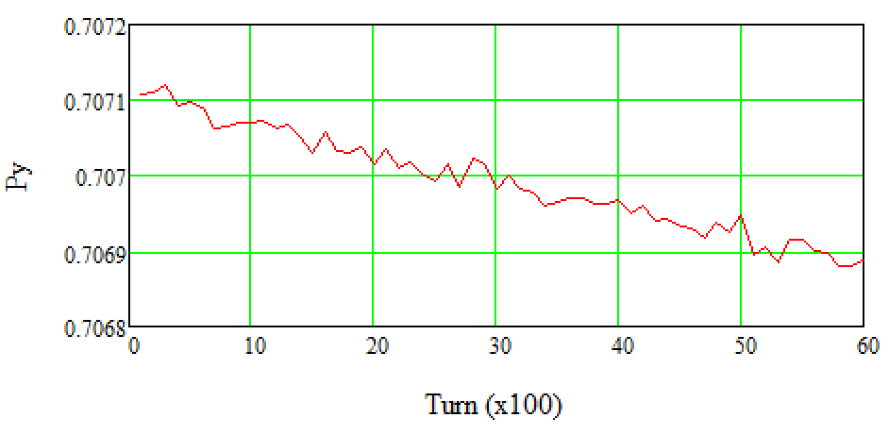
\includegraphics[width=0.9\linewidth]{2_polar1} \\ а)
    \end{minipage}
    \hfill
    \begin{minipage}[b][][b]{0.49\linewidth}\centering
        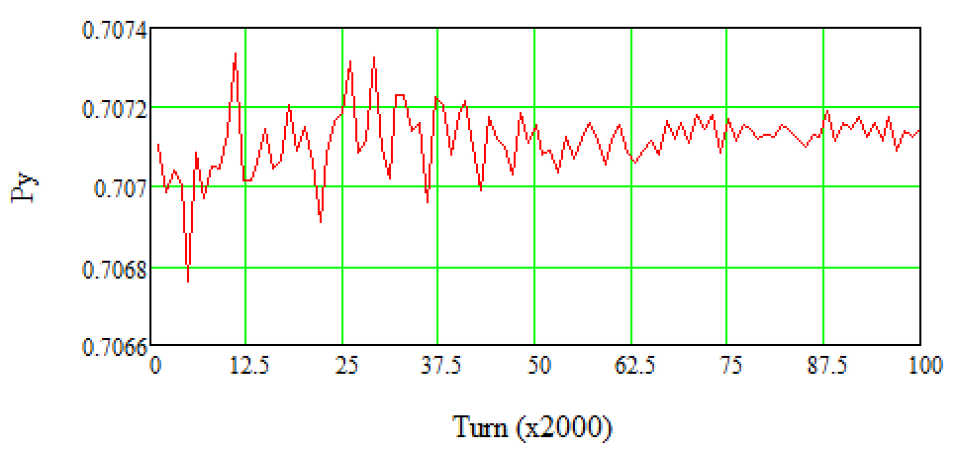
\includegraphics[width=0.9\linewidth]{2_polar2} \\ б)
    \end{minipage}
    \caption{Изменение поляризации во время процедуры скачка критической энергии: (а) ускорение на этапе 2, (б) скачок на этапе 3.}
\end{figure}

\par При моделировании рассматриваются частицы с различными доступными начальными параметрами. Инжир. на рисунке polar показано изменение поляризации на 2-м (2 раза по $10^5$ оборотов) и 3-м (6 раз по $10^3$ оборота) этапах процедуры перехода. Поляризация здесь определяется как сумма проекций вектора спина на ось Y всех частиц и существенно не менялась в ходе процедуры. Стоит отметить, что COSY Infinity позволяет отслеживать вектор спина только для небольшого числа частиц, а не для ансамбля, что плохо для изучения поляризации.

\par Более подробно спиновая динамика будет рассмотрена в ЭДМ-эксперименте всего комплекса NICA-Nuclotron в Главе 4.

\section*{Выводы}
\par Рассмотрена продольная динамика пучка вблизи критической энергии, а также при её пересечении. Такая особенность характерна для структуры, в которой энергия инжекции пучка меньше критической энергии установки и возникает необходимость её преодоления для ускорения до конечной энергии эксперимента.

\begin{enumerate}

\item Воздействие критической энергии на продольную динамику пучка вызывает увеличение фазового объёма в результате неадиабатичности и нелинейности движения в области энергии, близкой к критической;

\item Для преодоления критической энергии может быть применена процедура скачка, которая подразумевает кратковременное изменение дисперсионной функции. Это может быть достигнуто путём использования дополнительных квадруполей или квадруполей поворотной арки. В первом случае можно добиться сохранения частоты, а во втором — необходимо контролировать изменение рабочей точки и стабильность в поперечной плоскости. Таким образом, определяется величина и темп изменения критической энергии при проведении процедуры скачка;

\item Гармонический или барьерный тип ВЧ оказывает влияние на темп ускорения, а также продольное распределение внутри сепаратрисы. В сочетании со схемой процедуры скачка, необходимо сравнивать темп изменения критической энергии таким образом, чтобы относительный темп при пересечении критической энергии был в разы выше темпа ускорения;

\item Проведено исследование влияния простейших моделей импедансов на динамику. Результаты показали, что для интенсивных сгустков влияние импедансов оказывается значительным. Применение более точных моделей импедансов может существенно углубить понимание реальной динамики системы;

\item В условиях, близких к критическим для интенсивного пучка, развивается продольная микроволновая неустойчивость, которая существенно ограничивает характеристики пучка в конечном эксперименте и, в конечном счёте, приводит к уменьшению светимости в коллайдере.

\end{enumerate}


\FloatBarrier
